\documentclass[../main/main.tex]{subfiles}

\newdate{date}{02}{11}{2020}

% \begin{figure}[h!]
% \centering
% \includegraphics[page=6,width=0.8\textwidth]{../lessons/pdf_file/13_lecture.pdf}
% \end{figure}

%\displaydate{date}. Compiled:  \today. Alice.

\begin{document}

\pagestyle{plain}

\section{Lecture 13}


\subsubsection*{Slide 1}

\begin{minipage}[]{0.5\linewidth}
\centering
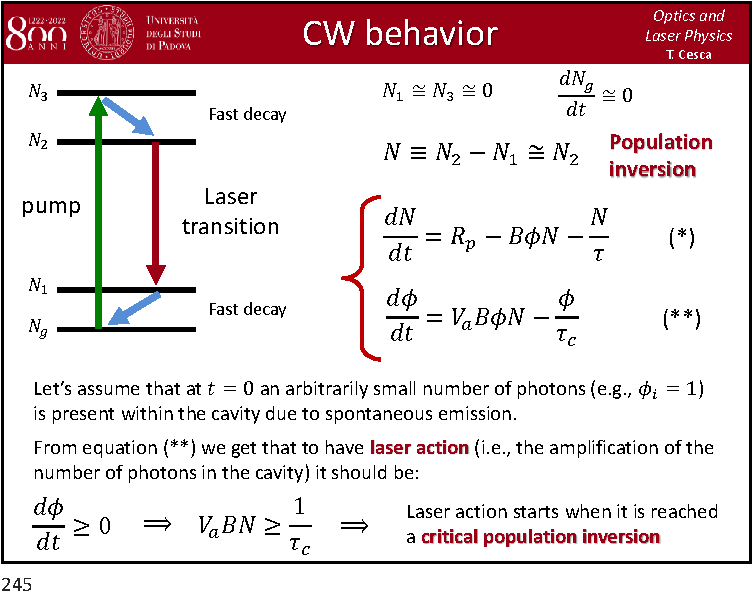
\includegraphics[page=1,width=1\textwidth]{../lessons/pdf_file/13_lecture.pdf}
\end{minipage}
\hspace{0.3cm}\vspace{0.3cm}
\begin{minipage}[c]{0.47\linewidth}

The expression for the output power is the same for a three-level system.

Let us assume that at \( t=0 \) there is a small number of photons within the cavity given by spontaneous emission.

In this case, from the second rate equation, in order to get laser action we need an amplification of the number of photons. We obtain a condition on the population inversion: we have to overcome a \textbf{critical population inversion}.

\end{minipage}

\subsubsection*{Slide 2}

\begin{minipage}[]{0.5\linewidth}
\centering
\includegraphics[page=2,width=1\textwidth]{../lessons/pdf_file/13_lecture.pdf}
\end{minipage}
\hspace{0.3cm}\vspace{0.3cm}
\begin{minipage}[c]{0.47\linewidth}

This critical value can be computed. The result obtained is already being obtained calculating the treshold condition when we have the same number of photon at the beginning and between a passage back and forth (?).

\end{minipage}

\subsubsection*{Slide 3}

\begin{minipage}[]{0.5\linewidth}
\centering
\includegraphics[page=3,width=1\textwidth]{../lessons/pdf_file/13_lecture.pdf}
\end{minipage}
\hspace{0.3cm}\vspace{0.3cm}
\begin{minipage}[c]{0.47\linewidth}

We can also determine the \textbf{critical pumping rate} in order to obtain the \emph{critical population inversion}. At the treshold there are no photon in the cavity (we neglect the single photon that we assume should be present by spontaneous emission).

\end{minipage}

\newpage

\subsubsection*{Slide 4}

\begin{minipage}[]{0.5\linewidth}
\centering
\includegraphics[page=4,width=1\textwidth]{../lessons/pdf_file/13_lecture.pdf}
\end{minipage}
\hspace{0.3cm}\vspace{0.3cm}
\begin{minipage}[c]{0.47\linewidth}

The critical pumping rate is the pumping rate that you need to apply to your system in order to balance spontaneous emission transition from the upper laser level.

\end{minipage}

\subsubsection*{Slide 5}

\begin{minipage}[]{0.5\linewidth}
\centering
\includegraphics[page=5,width=1\textwidth]{../lessons/pdf_file/13_lecture.pdf}
\end{minipage}
\hspace{0.3cm}\vspace{0.3cm}
\begin{minipage}[c]{0.47\linewidth}

If the pumping rate is larger than the critical pumping rate, the number of photons start to increase.
As we suppose it is independent on time, the number of photon in the cavity reach a steady-state \( \Phi _0 \) and also a steady-state of population inversion \( N_0 \).

\end{minipage}

\subsubsection*{Slide 6}

\begin{minipage}[]{0.5\linewidth}
\centering
\includegraphics[page=6,width=1\textwidth]{../lessons/pdf_file/13_lecture.pdf}
\end{minipage}
\hspace{0.3cm}\vspace{0.3cm}
\begin{minipage}[c]{0.47\linewidth}

Let us compute the rate equations at the steady-state.

We have \( N_0 = N_c \), so the population inversion remains equal to the initial population inversion when the laser starts! So it is important to remind that the \textbf{population inversion does not change anymore}!

The number of photon above treshold at the steady-state increases linearly with the pumping rate.

\end{minipage}

\newpage

\subsubsection*{Slide 7}

\begin{minipage}[]{0.5\linewidth}
\centering
\includegraphics[page=7,width=1\textwidth]{../lessons/pdf_file/13_lecture.pdf}
\end{minipage}
\hspace{0.3cm}\vspace{0.3cm}
\begin{minipage}[c]{0.47\linewidth}

Instead, below the treshold (there is no laser action), there are no photons by stimulated emission.

The evolution over time of the population inversion has an exponential trend with an asymptotic behavior. It is a linear function of the pumping rate.

\end{minipage}

\subsubsection*{Slide 8}

\begin{minipage}[]{0.5\linewidth}
\centering
\includegraphics[page=8,width=1\textwidth]{../lessons/pdf_file/13_lecture.pdf}
\end{minipage}
\hspace{0.3cm}\vspace{0.3cm}
\begin{minipage}[c]{0.47\linewidth}

Let us sump up the different regimes.

We can introduce the \textbf{over-threshold factor}: the ratio between the pumping rate and the critical pumping rate, so how much you are pumping above treshold.

So, when you pump the material \textbf{below threshold} the energy that you are giving to your system is stored in the active medium and is used to increase the population inversion.

Instead, \textbf{above threshold}, the energy is stored in the cavity, because its the number of photon within the cavity which is increasing when laser action starts.

\end{minipage}

\subsubsection*{Slide 9}

\begin{minipage}[]{0.5\linewidth}
\centering
\includegraphics[page=9,width=1\textwidth]{../lessons/pdf_file/13_lecture.pdf}
\end{minipage}
\hspace{0.3cm}\vspace{0.3cm}
\begin{minipage}[c]{0.47\linewidth}

Let us suppose we are above threshold.

The \textbf{beam area} is in general smaller than the \textbf{section of the active medium}.

We can rewrite the number of photons as a function of the power.

\end{minipage}

\subsubsection*{Slide 10}

\begin{minipage}[]{0.5\linewidth}
\centering
\includegraphics[page=10,width=1\textwidth]{../lessons/pdf_file/13_lecture.pdf}
\end{minipage}
\hspace{0.3cm}\vspace{0.3cm}
\begin{minipage}[c]{0.47\linewidth}

If you are designing a laser, the behavior is a \textbf{threshold one}.

We introduced for a four-level system the \textbf{saturation intensity} and we can simplify the expression for the output power.

\end{minipage}

\subsubsection*{Slide 11}

\begin{minipage}[]{0.5\linewidth}
\centering
\includegraphics[page=11,width=1\textwidth]{../lessons/pdf_file/13_lecture.pdf}
\end{minipage}
\hspace{0.3cm}\vspace{0.3cm}
\begin{minipage}[c]{0.47\linewidth}

The \textbf{laser slope efficiency} is the slope of the line in the plot.

We remember also the expression for the \textbf{optical} and \textbf{electrical} pumping.

\end{minipage}

\subsubsection*{Slide 12}

\begin{minipage}[]{0.5\linewidth}
\centering
\includegraphics[page=12,width=1\textwidth]{../lessons/pdf_file/13_lecture.pdf}
\end{minipage}
\hspace{0.3cm}\vspace{0.3cm}
\begin{minipage}[c]{0.47\linewidth}

We can use these expression to rewrite the critical pumping rate.

We can write an explicit expression for the \textbf{threshold power} \( P_{th} \).

\end{minipage}

\subsubsection*{Slide 13}

\begin{minipage}[]{0.5\linewidth}
\centering
\includegraphics[page=13,width=1\textwidth]{../lessons/pdf_file/13_lecture.pdf}
\end{minipage}
\hspace{0.3cm}\vspace{0.3cm}
\begin{minipage}[c]{0.47\linewidth}

The laser slope efficiency can be also rewritten in another form as the product of the \textbf{pumping efficiency},  \textbf{outcoupling efficiency} (fraction of photons that are extracted from the cavity, so is related to the losser of the outcoupling mirror wrt the total losses of the cavity), \textbf{laser quantum efficiency} (ratio between the energy of your photon and the minimum energy that you need to give to your system in order to pump to the upper laser level) and \textbf{transverse efficiency} (ratio between the beam size of the mode on the active medium divided by the section of the active medium, it say you what is the fraction of the active medium you are using with your mode).

The larger is the slope, the large is the power that you can obtain from a given pumping power.

\end{minipage}

\subsubsection*{Slide 14}

\begin{minipage}[]{0.5\linewidth}
\centering
\includegraphics[page=14,width=1\textwidth]{../lessons/pdf_file/13_lecture.pdf}
\end{minipage}
\hspace{0.3cm}\vspace{0.3cm}
\begin{minipage}[c]{0.47\linewidth}

Let us try to describe a real system and let us see how much we can describe it.

Let us consider a Fabry-Perot cavity. We have an \textbf{optical pumping with elliptical cavity}.
There are no elements to select the mode of oscillations, so we have \textbf{multimodal oscillation}.

If you relax the first hypothesis of having a single mode, you end up with an intensity distribution which is homogeneous both in the transverse and longitudinal direction. So, it is possible in any case to get a good agreement between the experimental results and what we calculate phenomenologically.

\end{minipage}

These are the experimental paramaters.

\subsubsection*{Slide 15}

\begin{minipage}[]{0.5\linewidth}
\centering
\includegraphics[page=15,width=1\textwidth]{../lessons/pdf_file/13_lecture.pdf}
\end{minipage}
\hspace{0.3cm}\vspace{0.3cm}
\begin{minipage}[c]{0.47\linewidth}

Let us compare the experimental values with the analytcal one.

Here there are the physical paramaters of the system.

With the physical paramaters of our system we can calculate the saturation intensity. We have to calculate also the logaritmic losses given by the outcoupling mirror.

If we compare the experimental expression with what we can calculate theroetically, we can obtain the size of the medium. It is smaller wrt we can calculate by the transverse section of the rod and the diameter.

\end{minipage}

\subsubsection*{Slide 16}

\begin{minipage}[]{0.5\linewidth}
\centering
\includegraphics[page=16,width=1\textwidth]{../lessons/pdf_file/13_lecture.pdf}
\end{minipage}
\hspace{0.3cm}\vspace{0.3cm}
\begin{minipage}[c]{0.47\linewidth}

We can also compare the power theoretical threshold with the experimental one. But, we need the logaritmic losses.

\end{minipage}

\subsubsection*{Slide 17}

\begin{minipage}[]{0.5\linewidth}
\centering
\includegraphics[page=17,width=1\textwidth]{../lessons/pdf_file/13_lecture.pdf}
\end{minipage}
\hspace{0.3cm}\vspace{0.3cm}
\begin{minipage}[c]{0.47\linewidth}

We need \( \gamma _i  \) and we can compute it experimentallly.

So, you can do an experiment in which you vary the outcoupling mirror and you measure the treshold power of your system. In this way, you can obtain a linear relationship.

\end{minipage}

\subsubsection*{Slide 18}

\begin{minipage}[]{0.5\linewidth}
\centering
\includegraphics[page=18,width=1\textwidth]{../lessons/pdf_file/13_lecture.pdf}
\end{minipage}
\hspace{0.3cm}\vspace{0.3cm}
\begin{minipage}[c]{0.47\linewidth}

The intercept is \( -2 \gamma _i  \). This is the most efficient way to determine experimentally the losses. Otherwise, you have to analyze your elements what are teh sizes and so on...

\end{minipage}

\subsubsection*{Slide 19}

\begin{minipage}[]{0.5\linewidth}
\centering
\includegraphics[page=19,width=1\textwidth]{../lessons/pdf_file/13_lecture.pdf}
\end{minipage}
\hspace{0.3cm}\vspace{0.3cm}
\begin{minipage}[c]{0.47\linewidth}

We can compare the experimental value of the laser slope efficiency with the value that we have calculated.

We can compute the pumping efficiency.

\end{minipage}

\subsubsection*{Slide 20}

\begin{minipage}[]{0.5\linewidth}
\centering
\includegraphics[page=20,width=1\textwidth]{../lessons/pdf_file/13_lecture.pdf}
\end{minipage}
\hspace{0.3cm}\vspace{0.3cm}
\begin{minipage}[c]{0.47\linewidth}

Let us compute the ratio between the critical inversion and the total population in our material.

\end{minipage}

\end{document}
